\begin{figure}[t]
    \centering
    \begin{subfigure}{0.49\linewidth}
        \centering
        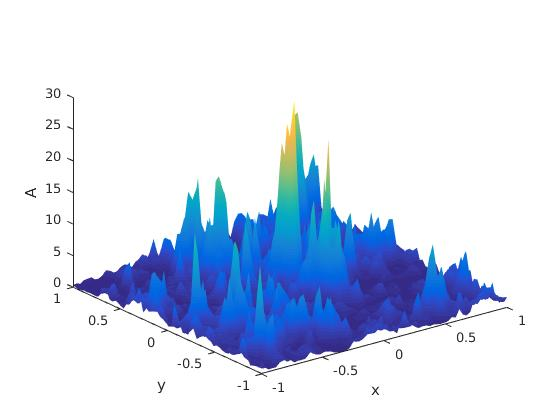
\includegraphics [width=1\linewidth]{Darcy/Pictures/A.jpg}
        \caption{Random field.}
        \label{fig:DarcyA}
    \end{subfigure}
    \begin{subfigure}{0.49\linewidth}
        \centering
        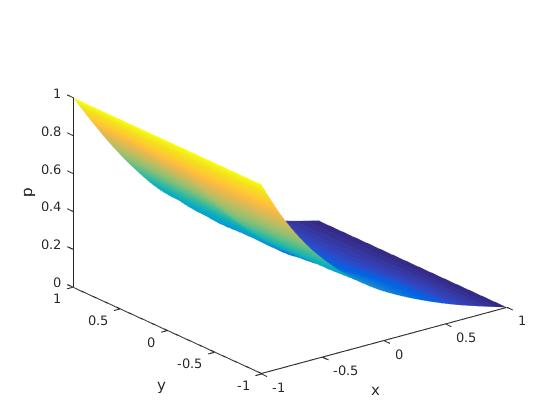
\includegraphics [width=1\linewidth]{Darcy/Pictures/P.jpg}
        \caption{Pressure field.}
        \label{fig:DarcyP}
    \end{subfigure}    
    \begin{subfigure}{0.49\linewidth}
        \centering
        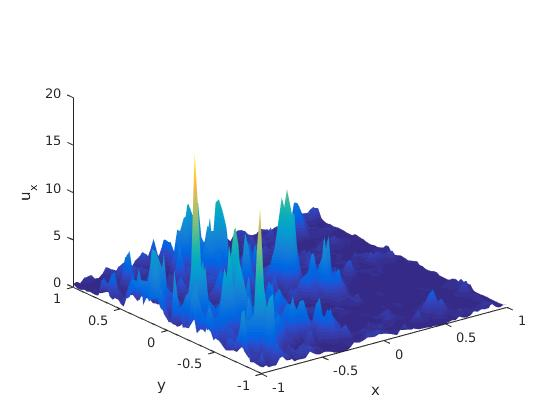
\includegraphics [width=1\linewidth]{Darcy/Pictures/Ux.jpg}
        \caption{$x$ component of velocity field.}
        \label{fig:DarcyUx}
    \end{subfigure}
    \begin{subfigure}{0.49\linewidth}
        \centering
        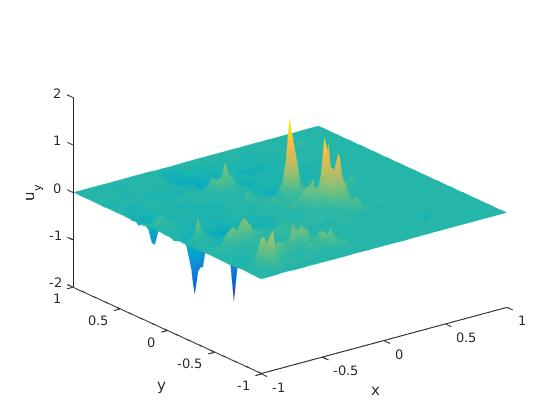
\includegraphics [width=1\linewidth]{Darcy/Pictures/Uy.jpg}
        \caption{$y$ component of velocity field.}
        \label{fig:DarcyUy}
    \end{subfigure}    
    \caption{Approximate solution of the uncertain Darcy problem.}
    \label{fig:DarcyResults}
\end{figure}

